\documentclass[paper=a4,11pt,parskip=half,toc=listof]{scrartcl}
\usepackage{report_package}


\begin{document}
%%%%%%%%%%%%%%%%%%%%% Startseite %%%%%%%%%%%%%%%%%%%%%%%%%%%
\begin{titlepage}
\begin{minipage}[t]{0.5\textwidth}
\begin{Large}
    \begin{flushleft}
      \hspace{1cm} \makebox[3cm][c]{
\includegraphics[height=8ex]{./logos/logo_hbrs.png} \vspace{1.8cm}}
    \end{flushleft}
\end{Large}
\end{minipage}

\vspace{0.07\textheight}
\begin{center}
 \begin{Large} \textbf{\ThesisUniversityCourse} \end{Large}\\
 \vspace{1em}
 \begin{Large} \textbf{-- \ThesisSemester --} \end{Large}\\
 \vspace{2em}
 \begin{Huge} \begin{spacing}{1.3} \textbf{\ThesisTitle} \end{spacing} \end{Huge}
 \vspace{2em}
 \begin{Large} \textbf{-- Report on dataset creation --} \end{Large}\\
 \vspace{2em}
  \begin{Large}\textbf{by} \end{Large}\\
 
 \vspace{2em}
 \begin{Large}\textbf{\ThesisAuthora}\end{Large}\\
 \begin{small}naresh.gurulingan@smail.inf.h-brs.de\end{small}\\
 \begin{small} Matr. no. 9030384\end{small}\\
\end{center}
\end{titlepage}

\newgeometry{top=4cm, bottom=3cm, left=4.5cm, right=3cm}

\newpage
\setcounter{page}{3} 
\begin{spacing}{1.14}
\tableofcontents
\end{spacing}

\clearpage{}
\listoftables % add list of tables
\clearpage{}
\listoffigures % add list of figures 
\clearpage{}
\include{acronym} % include the acronym thing
\clearpage{}

\setcounter{tocdepth}{4} 
\setcounter{secnumdepth}{4}
\setlength\parindent{0pt}  %indent disabled

\pagenumbering{arabic} % arabic numbers for the main part


\newpage
\section{Overview of the dataset}
Since semantic segmentation using deep learning is framed as a pixelwise classification task, an image of dimensions H$\times$W$\times$C requires a ground truth of dimensions H$\times$W, where H and W are the height and width of the image in the dataset having C number of channels. 

The scope of the dataset is to include objects associated to RoboCup @Work. The selected 18 objects are shown below:

Each of the objects were taken individually, placed on 3 different backgrounds and 30 images were taken. This lead to a total of 540 images which were to be manually labeled. Since, every pixel of the images needs to be labeled, the process of manual annotation would be time consuming. Therefore, a decision was made to first annotate the 540 images and later decide whether more images could be taken based on the effort required for annotation.

\section{Selection of a labeling tool}
In order to reduce the time required to annotate an image, it was imperative to select a tool which is specifically designed for semantic segmentation and also provides algorithms which helps the annotator by providing labeling automation to the highest possible extent.

The following available tools were evaluated for ease of use and time taken for annotation:
	\begin{itemize}
		\item LabelMe: web based tool is public and data would also be public.
		\item LabelMe Matlab toolbox: yet to try..
		\item University bonn annotation tool:
		\item Pixel annotation tool (using watershed algorithm): works in windows. Seems to be useful.
		\item Ratsnake: tool dint seem to be useful although the website had options like superpixel suggestions.
		\item LabelImg: Can be used but time consuming.
		\item Figi: used in medical image segmentation. Has many options. Still exploring.
		\item Supervisely.
		\item MATLAB ImageLabeler available in release R2017b (Computer Vision Toolbox).
	\end{itemize}

\section{Description of the labeling process}
\label{section:process}
MATLAB ImageLabeler was used for the labeling process. At first, label definitions are created and exported to a .mat file. This file is used to load label definitions for all images to maintain consistency of labels. The contents of the .mat file is shown in the figure\ref{Fig:2}.

	\begin{figure}[htb!]
		\centering
		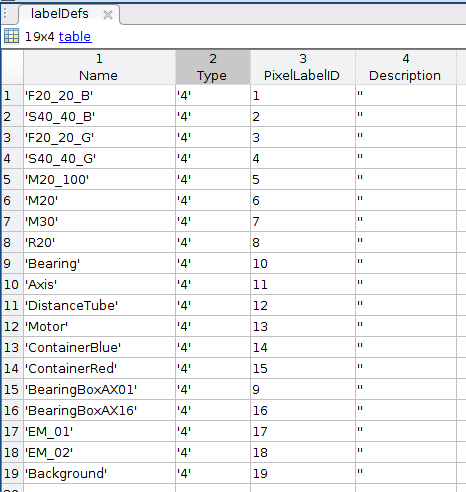
\includegraphics[scale=0.7]{labelDef}
		\caption{Contents of the labelDefs .mat file}
		\label{Fig:2}
	\end{figure}
	
The ImageLabeler app, by default, provides different tools which help create pixelwise labels\ref{Fig:3}. These tools become accessible once an image and the label definitions are loaded. A short description of the tools is given below:
	\begin{figure}[htb!]
		\centering
		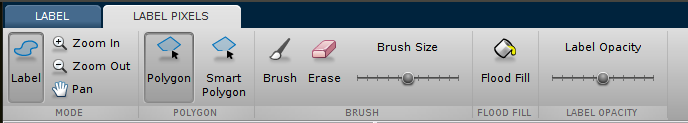
\includegraphics[scale=0.55]{label_tools}
		\caption{Tools provided by the ImageLabeler app}
		\label{Fig:3}
	\end{figure}
	
	\begin{itemize}
		\item Polygon: This can be used to trace an object boundary by placing dots. Once a closed contour is created, pixels within the contour get assigned the corresponding object label.
		\item Smart Polygon: Can be used in a similar fashion like the Polygon tool. This tool, in addition, tries to reach out to the nearby edges of the drawn polygon.
		\item Brush and Erase: Square shaped brush and eraser to either label a region or remove labels from a region. The size of the square can be changed by using the Brush Size slider.
		\item Flood Fill: This tool provides same labels to pixels which are similar in terms of the intensity with the selected pixel.
		\item Label Opacity: This tool provides a sliding bar which varies the opacity of the overlayed labels on the image. This is helpful to visualize the assigned labels.
		\item Zoom In, Zoom Out, Pan: These tools improve the ease of labeling by providing means to focus on particular regions by zooming and panning.
	\end{itemize}
	
The ImageLabeler app by default assigns different colors to different objects to aid visualization. The label colors are shown in the ROI Label Definition window\ref{Fig:4}.
	\begin{figure}[htb!]
		\centering
		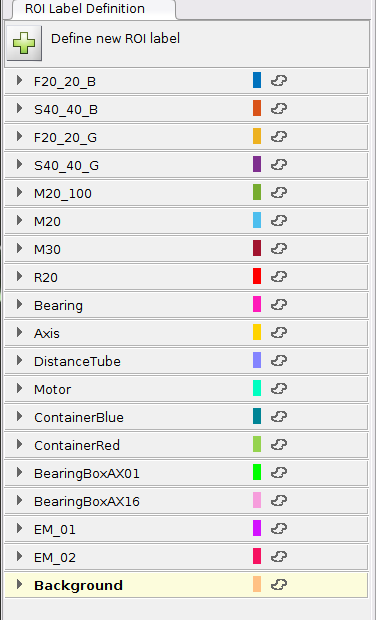
\includegraphics[scale=0.6]{roi_label_defintions}
		\caption{ROI Label Definitions window}
		\label{Fig:4}
	\end{figure}
	
The ImageLabeler app does not provide any tool to label all unlabeled pixels as background. In order to save time, each of the images taken, only have one object

In order to save time, the following workarounds have been used:
	\begin{itemize}
		\item The images taken for the dataset each have only one object in them.
		\item Only the object region is labeled.
		\item Since the ImageLabeler app does not provide any tool to label all unlabeled pixels as background, a python code which simply reads the label image and replaces unlabeled values 0 with background label value 19, was used for this purpose. The code is also used to double check the label image in order to avoid noisy labeling.
	\end{itemize}
	
The Export Labels -> To File option can be used to save the annotations. This is done for all images individually to arrive at the folder structure shown in \ref{Fig:5a}:
	
The saved .mat file can be loaded into ImageLabeler again to further modify labels if required later. The 'Label\_1.png' file located in the PixelLabelData folder (as can be seen in \ref{Fig:5a}) is the label image. This image is renamed to have the same name as the image file and the following folder structure is created by using a python code\ref{Fig:5b}.
	
\begin{center}
	\begin{figure}[!htb]
		\begin{subfigure}{.5\textwidth}
			\centering
			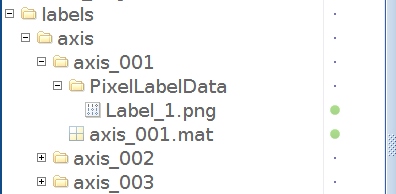
\includegraphics[width=1\linewidth]{folder_structure}
			\caption{Folder structure of saved labels}
			\label{Fig:5a}
		\end{subfigure}
		\begin{subfigure}{.5\textwidth}
			\centering
			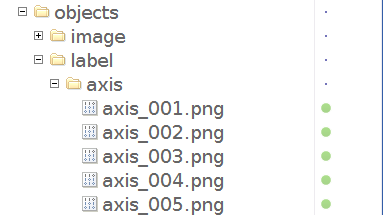
\includegraphics[width=1\linewidth]{folder_structure_aug}
			\caption{Rearranged folder structure}
			\label{Fig:5b}
		\end{subfigure}
		\caption{Different folder structures}
		\label{Fig:5}
	\end{figure}
\end{center}

The final folder structure is shown in \ref{Fig:6}. The image folder and label folder are similar and contain object images and corresponding label images with same names.

\begin{center}
	\begin{figure}[!htb]
		\begin{subfigure}{.5\textwidth}
			\centering
			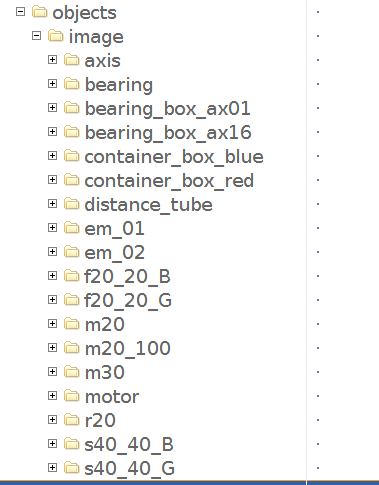
\includegraphics[width=1\linewidth]{folder_image}
			%\caption{}
			\label{Fig:6a}
		\end{subfigure}
		\begin{subfigure}{.5\textwidth}
			\centering
			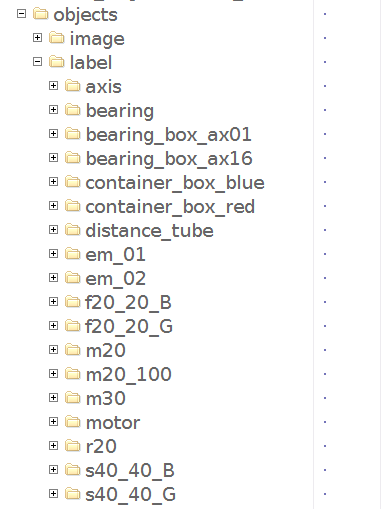
\includegraphics[width=1\linewidth]{folder_label}
			%\caption{}
			\label{Fig:6b}
		\end{subfigure}
		\caption{Folder structure showing different object folders in both image and label folders.}
		\label{Fig:6}
	\end{figure}
\end{center}

\section{About the augmentation script}
\subsection{Motivation}
	\begin{itemize}
		\item Manually labeling 540 images with the described process in \ref{section:process} takes roughly 2160 minutes (roughly 4 minutes per image). This is equivalent to around 4 working days. Hence, creating a large dataset with manual labeling is not feasible.
		\item Taking images in a variety of real world backgrounds is also time consuming.
		\item Labeling images with multiple objects would take an even longer time.
	\end{itemize}
	
These drawbacks could be overcome by randomly placing objects on a variety of different background images.



\section{Meta-data of the dataset}



\section{Conclusion and possible directions of improvement}
	\begin{itemize}
		\item Improve the way in which PixelLabelData is saved.
		\item Integrating 'rest of the pixels are background' into MATLAB ImageLabeler.
		\item Integration of augmentation script with MATLAB ImageLabeler.
		\item GUI for the augmentation script.
	\end{itemize}

\newpage
\addcontentsline{toc}{section}{References}
\begin{thebibliography}{9}
\bibitem{1}

\end{thebibliography}
\end{document}
